%%%%%%%%%%%%%%%%%%%%%%%%%%%%%%%%%%%%%%%%%%%%%%%%%%%%%%%%%
\section{Scenario}
\label{sec:rules:scenario}
Most tests take place in the \RoboCup\AtHome{} \Arena{}. Some tests can take place outside, in a previously unknown public place (see~\ref{sec:concepts:nonstandardscenario}). This section describes the \Arena{} and how it is furnished,  as well as, known information that is shared in all tests. 

\subsection{RoboCup@Home Arena}
\label{sec:rules:scenario:arena}
The \RoboCup\AtHome{} \Arena{} is a realistic home setting consisting of inter-connected rooms.
The minimal configuration consists of:
\begin{itemize}
	\item Bedroom
	\item Dining Room
	\item Living Room
	\item Kitchen
\end{itemize}
% There is one \Arena{} for each league and an additional one for setup and training shared by all leagues.

An \Arena{} is decorated and dressed to resemble a typical apartment in the hosting country/region, including all necessities and decorations one can find in a normal house.

\subsection{Walls, Doors and Floor}
\label{sec:rules:scenario:walls}
The indoor home setting will be surrounded by high and low walls built up using standard fair construction material.

\begin{itemize}
	\item \textbf{Walls:} Walls have a minimum height of \SI{60}{\centi\meter}. A maximum height is not specified, but the audience must be able to watch the competition.

	\item \textbf{Doors:} There will be at least two doors, leading in and out of the arena.
	Inside the arena, rooms are connected by doors (at least one).
	All doors have handles, not knobs.
	Doors can be closed during tests, robots are expected to open them or plan around.

	\item \textbf{Floor:} The floor and doorways of the arena are even.
	There will be no significant steps or even stairways.
	Minor unevenness such as carpets, transitions in floor covering between different areas, and minor gaps (especially at doorways) can be expected.

	\item \textbf{Appearance:} Floor and walls are mainly uni-colored but can contain texture, e.g., a carpet on the floor, a poster or picture on the wall.\\
\end{itemize}


\subsection{Furniture}
\label{sec:rules:scenario:furniture}
The arena will be furnished with items common in the host country.

The minimal configuration consists of:
\begin{itemize}
	\item Bed,
	\item Couch
	\item Small Table
	\item Small Dinner Table with Two Chairs
	\item Two Trash Bins
	\item Television with Remote Control
	\item Cupboard with Drawers
	\item Bookcase
	\item Coat Rack
\end{itemize}

The \Arena\textit{'s} kitchen must have:
\begin{itemize}
	\item Dishwasher
	\item Sink
	\item Powered Refrigerator (with some cans and plastic bottles inside).
\end{itemize}

A typical arena setup is shown in~\reffig{fig:scenario_arena}.

\begin{figure}[H]
	\centering
	\subfloat[Typical arena]{\label{fig:scenario_arena}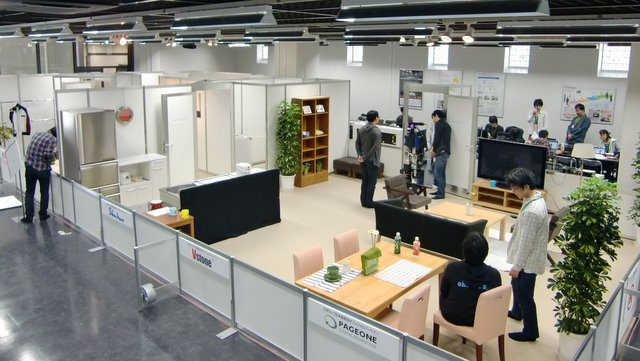
\includegraphics[height=46mm]{images/typical_arena.jpg}} ~
	\subfloat[Typical objects]{\label{fig:scenario_objects}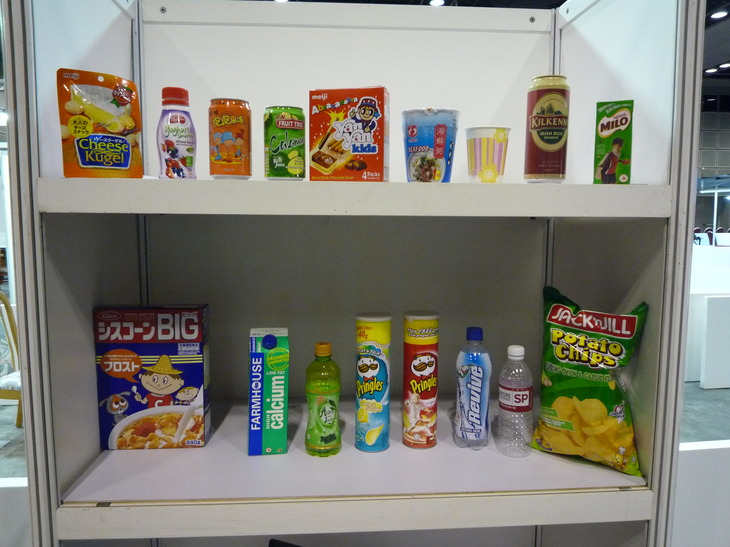
\includegraphics[height=46mm]{images/typical_objects.jpg}}
	\caption{Example \RoboCup\AtHome{} scenario.}
	\label{fig:arena}
\end{figure}

\subsubsection{Cupboard}
The cupboard can be any shelf-like furniture in which objects can be placed. At least one shelf must be lower than \SI{90}{\cm}.

\subsubsection{Fridge}
Fridge must not be smaller than \SI{120}{\cm}. At least one powered and functioning fridge is required.

\subsection{Objects}
\label{sec:rules:scenario:objects}
Some tests involve recognizing and manipulating objects (See~\reffig{fig:scenario_objects}).
The \TC{} will compile a list of at least \NumObjects{} objects at the competition. This list contains a picture of the object, as well as, its official name and \ObjectCategory{}. Every \ObjectCategory{} has an assigned \PredefinedLocation{} (see \ref{sec:rules:scenario:locations}) where objects of that category can usually be found during tests.
Each object is provided at the competition for training.

There are two types of objects:

\begin{enumerate}
	\item \textbf{\KnownObjects{}:} Objects previously known by the robot.%, split into:
% 	\begin{enumerate}
% 		\item \textbf{\ConsistentObjects{}:} Objects that always look the same.
% 		\item \textbf{\SimilarObjects{}:} Objects that look different to the provided image but are still considered the same by people (e.g. differently colored apple, cloth with different pattern).
% 		\item \textbf{\StandardObjects{}:} Objects chosen from the \YCBData{}\footnote{\url{http://www.ycbbenchmarks.com/object-set/}}. They are published 6 months in advance on the \RoboCup\AtHome{} website\footnote{\url{https://athome.robocup.org/standard-objects}} so that they can be aquired and trained beforehand.
% 	\end{enumerate}
	\item \textbf{\UnknownObjects{}:} Any other object that is not in the object list but can be grasped or handled (e.g. arena decorations).
\end{enumerate}

Known objects include at least:
\begin{itemize}
	\item \textbf{\iterm{Tableware}:} Dish, bowl, cup, and napkin (See~\reffig{fig:scenario_container_bowl}).
	\item \textbf{\iterm{Cutlery}:} Fork, knife, and spoon.
	\item \textbf{\iterm{Trash Bags}:} Big plastic trashbags, preferrably with handle.
	\item \textbf{\iterm{Bags}:} Lightweight. With stiff, vertical handles (See~\reffig{fig:scenario_container_bag}).
	\item \textbf{\iterm{Trays}:} Tray or basket, intended for two-handed manipulation (See~\reffig{fig:scenario_container_tray}).
	\item \textbf{\iterm{Pourable}:} An object whose content can be poured (e.g.~jug).
	\item \textbf{\iterm{Heavy Object}:} Weight between 1.0kg and 1.5kg (e.g.~water bottle).
	\item \textbf{\iterm{Tiny Object}:} A lightweight object, no bigger than 5cm (e.g.~teabag).
	\item \textbf{\iterm{Fragile Object}:} An easy-to-break object (e.g.~egg).
	\item \textbf{\iterm{Deformable Object}:} A flexible object that may appear in different shapes (e.g.~cloth).
\end{itemize}

\begin{figure}[H]
	\centering
	\subfloat[Brightly colored paper bags]{
		\label{fig:scenario_container_bag}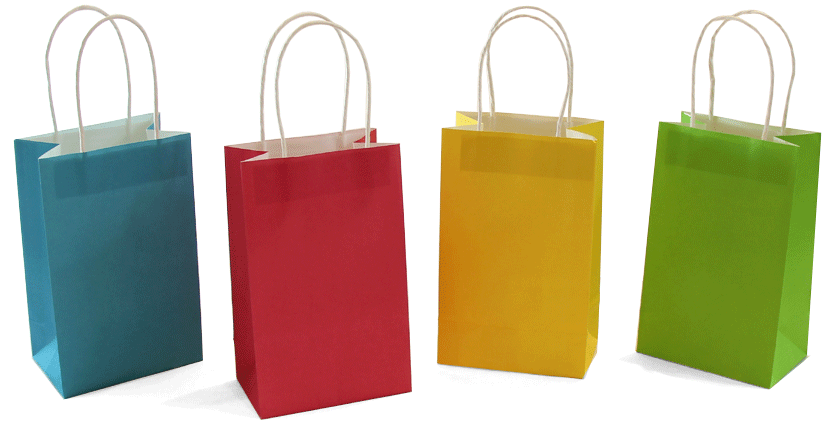
\includegraphics[width=0.33\textwidth]{images/container_paper_bag.png}}~
	\subfloat[Cereal bowls]{
		\label{fig:scenario_container_bowl}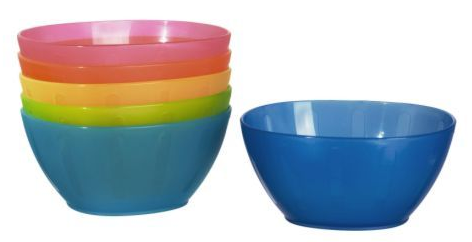
\includegraphics[width=0.33\textwidth]{images/container_bowl.png}}~
	\subfloat[Serving tray]{
		\label{fig:scenario_container_tray}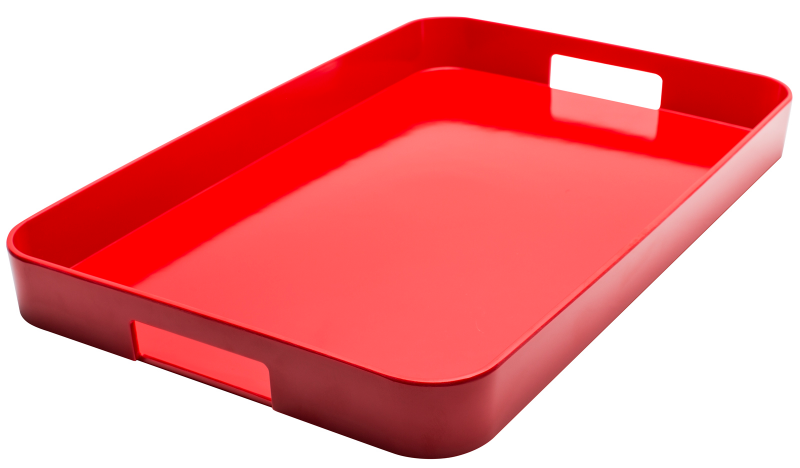
\includegraphics[width=0.33\textwidth]{images/container_tray.png}}
	\caption{Example of objects}
	\label{fig:scenario_containers}
\end{figure}

\noindent During the competition, objects can be requested based on their \ObjectCategory{}, physical attributes, or a combination of both.
Relevant attributes to be used are:
\begin{itemize}
	\item Color (e.g. red, blue, black with white dots, etc.).
	\item Relative estimated size (smallest, largest, big one, etc.).
	\item Relative estimated weight (lightest, heaviest).
	\item Relative position (left of, right most, etc.).
	\item Object description (is fragile, is container, can be poured, requires two hands, etc.).
\end{itemize}

\noindent\textbf{Remark:} Measurements are estimations and based on common sense. It is OK for robots to consider similar objects to be about the same size or weight. Don't bring a scale.


\subsection{Changes to the Arena}
\label{sec:rules:scenario:changes}
Since the robots should be able to function in the real world, the \Arena{} is not fixed and might change without further notice.
\begin{enumerate}
	\item \textbf{Major Changes:}
	Any furniture (\PredefinedLocation{} or not) might be moved slightly between tests. It will not change rooms or move drastically inside a room. However, a couch or table may be rotated, moved to its side etc. Walls will stay in place and rooms will not change function. Passages might be blocked.
	
	\item \textbf{Minor Changes:} Slightly moved chairs, slightly closed doors, or anything similar cannot be avoided and might happen at any time, even during a test.
\end{enumerate}

\noindent Only during \SetupDays{} (see~\ref{chap:setupdays}), teams can make changes to the arena if something severely hinders the robots (e.g. high door steps). These changes must be agreed upon by all team leaders and in accordance with the \TC{} on location.

During \SetupDays{} and in between tests, teams can take objects from the \Arena{} for training. A team may not take more than five objects at once and for longer than an hour. Teams may not modify any of the objects. At least half an hour before a test slot, all items must be returned to the \Arena{}.


\subsection{Predefined Rooms and Locations}
\textit{\label{sec:rules:scenario:locations}}
Some tests involve a \PredefinedLocation{}.
\begin{itemize}
	\item \textbf{Rooms:} Each room has a function (e.g. kitchen, bed room).
	
	\item \textbf{Furniture:} Some furniture will be named and sorted into a location class (e.g. couch and arm chair are both in the seating class). 
	
	\item \textbf{Doors:} Two doors leading in and out of the \Arena{} will be named entrance and exit respectively.
\end{itemize}


\subsection{Predefined Names}
\label{sec:rules:scenario:names}
Some tests involve memorizing a person's name. All people in the arena have an assigned \PredefinedName{} chosen from a list compiled by the \TC{}. This list has \NumNames{} names of which \SI{50}{\percent} are male and \SI{50} {\percent} female,
%, and \SI{50}{\percent} gender-neutral,
taken from the list of most common used names in the United States \footnote{\url{https://www.ssa.gov/oact/babynames/decades/century.html}}.


% \subsection{Wireless Network}
% \label{sec:rules:scenario:wifi}

% For wireless communication, an \ArenaNetwork{} is provided. The actual infrastructure depends on the \LOC{}. Reliability and stability is not guaranteed. Robots are expected to run regardless.

% The following rules apply:

% \begin{itemize}
% 	\item Only the \ArenaNetwork{} can be used by robots during tests.
% 	\item Only the active team in a test is allowed to use the \ArenaNetwork{}.
% 	\item One Virtual Local Area Networks (VLANs) is provided per team.
% 	\item Each VLAN is most likely to have its own SSID/password.
% 	\item VLAN traffic is separated from any other team, routed to the team's network cable in the team area.
% 	\item Each VLAN is also connected to the Internet.
% \end{itemize}

% \noindent Teams broadcasting unauthorized (aka rogue) wireless networks will be disqualified from the competition, and have their devices confiscated by the OC. This includes smartphones and concealed SSIDs. It is advised to verify your devices.
% \\ \\
% \textbf{Note:} All information about the scenario will be announced during \SetupDays{} (see~\ref{chap:setupdays}).

% Local Variables:
% TeX-master: "../Rulebook"
% End:
